% =====================================================================
%  RELATÓRIO - LABORATÓRIO DE PROCESSADORES
%  Sistema de Controle de Acesso Veicular com Raspberry Pi
%

%  As referências ficam no arquivo externo referencias.bib
%
%  Compilar com:
%     pdflatex relatorio
%     bibtex   relatorio
%     pdflatex relatorio
%     pdflatex relatorio
% =====================================================================

\documentclass[11pt,a4paper]{article}

% ---------- Codificação e idioma ----------
\usepackage[utf8]{inputenc}
\usepackage[T1]{fontenc}
\usepackage[brazil]{babel}
\usepackage{lmodern}
\usepackage{microtype}

% ---------- Layout ----------
\usepackage[a4paper,margin=2.5cm]{geometry}
\usepackage{setspace}
\onehalfspacing
\usepackage{indentfirst}
\usepackage{parskip}

% ---------- Recursos ----------
\usepackage{graphicx}
\usepackage{float}
\usepackage{booktabs}
\usepackage{longtable}
\usepackage{array}
\usepackage{enumitem}
\usepackage{xcolor}
\usepackage{tikz}
\usetikzlibrary{arrows.meta, positioning}
\usepackage{caption}
\usepackage[numbers,sort&compress]{natbib}
\usepackage[hidelinks]{hyperref}

% Citações numéricas no estilo [1]. Para formatação ABNT (autor-data),
% substitua as duas linhas de natbib/bibliographystyle por:
%   \usepackage[alf]{abntex2cite}   e   \bibliographystyle{abntex2-alf}

% ---------- Cores ----------
\definecolor{cinzaclaro}{RGB}{240,240,240}
\definecolor{cinzamedio}{RGB}{150,150,150}
\definecolor{laranja}{RGB}{200,90,0}

% ---------------------------------------------------------------------
%  MACROS DE APOIO
% ---------------------------------------------------------------------

% Marca um trecho que ainda precisa ser preenchido pelo grupo.
\newcommand{\pendencia}[1]{%
  \textcolor{laranja}{\textbf{[A COMPLETAR:} \textit{#1}\textbf{]}}%
}

% Lacuna curta para células de tabela que receberão um número.
\newcommand{\vazio}{\textcolor{laranja}{\rule[-1pt]{1cm}{0.6pt}}}

% Caixa cinza que ocupa o lugar de uma foto/figura ainda inexistente.
% Uso: \figplaceholder{largura}{altura}{texto explicativo}
\newcommand{\figplaceholder}[3]{%
  \begin{tikzpicture}
    \draw[dashed, cinzamedio, fill=cinzaclaro] (0,0) rectangle (#1,#2);
    \node[text width=#1cm-1cm, align=center, cinzamedio]
      at (#1/2,#2/2) {\small\textit{#3}};
  \end{tikzpicture}%
}

\newcolumntype{L}[1]{>{\raggedright\arraybackslash}p{#1}}

% =====================================================================
\begin{document}

% ---------------------------------------------------------------------
%  CAPA
% ---------------------------------------------------------------------
\begin{titlepage}
\centering

\vspace*{1cm}

{\large Escola Politécnica da Universidade de São Paulo}\\[0.3cm]
{\large Laboratório de Processadores}\\[0.3cm]
{\large PCS3732}

\vspace{3.5cm}

{\Huge\bfseries Sistema de Controle de Acesso Veicular\par}
\vspace{0.6cm}
{\LARGE Autenticação por RFID com Segundo Fator Noturno\par}
\vspace{3cm}

\begin{tabular}{ll}
\toprule
\textbf{Integrante} & \textbf{NUSP} \\
\midrule
Túlio Fogaça Panza              & 14609940 \\
Daniel Henrique Braga da Silva  & 14565432 \\
Caio Moussa Assumpção           & 12553966 \\
\bottomrule
\end{tabular}

\vspace{2cm}

{\normalsize Professor(a): Victor Takashi Hayashi}\\[0.3cm]

\vfill

\begin{minipage}{0.9\textwidth}
\centering\small
\textbf{Repositório:} \url{https://github.com/TulioPz/projeto_lab_proc}\\[0.2cm]
\end{minipage}
\end{titlepage}

% =====================================================================
\section{Introdução}
% =====================================================================

\subsection{Contextualização e motivação}

O controle de acesso de veículos é uma necessidade recorrente em estacionamentos
corporativos, condomínios e instituições de ensino. Soluções manuais, baseadas em
porteiros ou em cartões de papel, apresentam custo operacional elevado, são
suscetíveis a erros humanos e não produzem registros confiáveis sobre quem entrou
e quando. Sistemas automatizados baseados em identificação por radiofrequência
(RFID) oferecem uma alternativa de baixo custo, rápida e auditável, sendo hoje a
tecnologia predominante nesse tipo de aplicação. As credenciais empregadas neste
projeto seguem o padrão de proximidade definido pela norma
ISO/IEC~14443~\cite{iso14443}.

Entretanto, a autenticação por um único fator --- a posse da credencial física ---
é vulnerável: uma tag perdida, clonada ou emprestada concede acesso irrestrito.
Esse risco é agravado em períodos de baixa ocupação, quando não há testemunhas
nem vigilância presencial. A proposta deste projeto parte justamente dessa
observação: adotar autenticação de fator único durante o horário comercial,
privilegiando a fluidez do trânsito de veículos, e exigir um segundo fator
(senha digitada em teclado matricial) no período noturno, quando o risco é maior
e o volume de acessos é baixo o suficiente para tolerar o tempo adicional de
autenticação. Essa combinação de um fator de posse com um fator de conhecimento
segue a prática recomendada para autenticação multifator~\cite{nistmfa}.

\subsection{Objetivos}

O objetivo geral é desenvolver um sistema embarcado, executado em uma Raspberry
Pi, capaz de controlar de forma autônoma e segura a entrada e a saída de veículos
em um estacionamento corporativo. Como objetivos específicos, destacam-se:

\begin{enumerate}[itemsep=1pt]
  \item identificar veículos por meio de tags RFID e validar sua autorização;
  \item aplicar autenticação de dois fatores no período noturno;
  \item acionar uma cancela simulada por servomotor, com abertura e fechamento
        controlados;
  \item detectar a passagem do veículo por sensor ultrassônico, impedindo o
        fechamento da cancela sobre o veículo;
  \item manter de forma persistente o registro dos veículos presentes no
        estacionamento, permitindo distinguir automaticamente operações de
        entrada e de saída;
  \item manter um histórico de entradas e saídas com identificação do usuário,
        data e horário de cada acesso;
  \item tratar falhas de sensores e de leitura de forma segura, evitando
        movimentos da cancela quando o estado do sistema não puder ser
        determinado com segurança.
\end{enumerate}

\subsection{Escopo desta entrega}

Este relatório documenta a versão final desenvolvida para o protótipo. O sistema
integra leitor RFID, display LCD, servomotor, sensor ultrassônico e teclado
matricial em um único fluxo de controle executado pela Raspberry Pi. Além da
autenticação diferenciada entre os períodos diurno e noturno, a versão final
incorpora armazenamento persistente do estado dos veículos e um histórico de
entradas e saídas.

No protótipo, uma única cancela física é utilizada para representar os dois
sentidos de circulação. Após a leitura de uma tag válida, o sistema consulta o
registro persistente: se o veículo não estiver presente, a operação é tratada
como entrada; se já estiver presente, a nova leitura é interpretada como saída.
Uma segunda cancela física dedicada exclusivamente à saída permanece como
possível evolução da montagem. A sinalização sonora por buzzer também não foi
integrada à versão final.

% =====================================================================
\section{Especificação de Requisitos}
% =====================================================================

\subsection{Requisitos funcionais}

\begin{longtable}{@{}p{1.3cm}L{9.5cm}p{3.3cm}@{}}
\caption{Requisitos funcionais e situação atual.}\label{tab:rf}\\
\toprule
\textbf{ID} & \textbf{Descrição} & \textbf{Situação} \\
\midrule
\endfirsthead
\toprule
\textbf{ID} & \textbf{Descrição} & \textbf{Situação} \\
\midrule
\endhead
\bottomrule
\endfoot

RF01 & Ao aproximar uma tag do leitor, o sistema verifica se seu identificador
consta na lista de usuários autorizados; caso contrário, a entrada é recusada.
& Implementado \\[4pt]

RF02 & O sistema deve permitir cadastrar e descadastrar tags.
& Não implementado dinamicamente \\[4pt]

RF03 & O sistema deve identificar se o acesso ocorre em período diurno ou
noturno, prioritariamente pelo relógio do sistema.
& Implementado \\[4pt]

RF04 & No período diurno, uma tag válida é suficiente para autorizar a entrada.
& Implementado \\[4pt]

RF05 & No período noturno, exigem-se dois fatores: tag válida e senha correta
digitada em teclado matricial.
& Implementado \\[4pt]

RF06 & O sistema controla a abertura e o fechamento da cancela por servomotor.
& Implementado \\[4pt]

RF07 & Um sensor ultrassônico detecta a presença e a passagem do veículo na
região da cancela.
& Implementado \\[4pt]

RF08 & Após a passagem completa do veículo, a cancela retorna à posição fechada;
o fechamento não ocorre enquanto houver detecção de presença.
& Implementado \\[4pt]

RF09 & Após uma entrada bem-sucedida, o sistema atualiza o registro persistente
de veículos presentes e acrescenta a operação ao histórico de acessos.
& Implementado \\[4pt]

RF10 & O sistema mantém a relação dos veículos atualmente dentro do
estacionamento.
& Implementado \\[4pt]

RF11 & Uma nova leitura de RFID para um veículo já registrado como presente
deve ser interpretada como solicitação de saída.
& Implementado \\[4pt]

RF12 & Após a saída, o veículo deve ser removido do registro de presença e a
operação deve ser acrescentada ao histórico com data e horário.
& Implementado \\[4pt]

RF13 & Tag não cadastrada: negar acesso, manter a cancela fechada e informar o
usuário.
& Implementado \\[4pt]

RF14 & Senha incorreta no período noturno: negar acesso e manter a cancela
fechada, com limite de tentativas consecutivas.
& Implementado \\[4pt]

RF15 & Falha do sensor ultrassônico: impedir o fechamento enquanto não houver
confirmação segura de que a área de passagem está livre.
& Implementado \\[4pt]

RF16 & Falha do leitor RFID: manter a cancela fechada e impedir autorização
automática.
& Implementado \\[4pt]

RF17 & Sinalização sonora por buzzer para eventos como acesso autorizado, acesso
negado e erro do sistema. \textit{(opcional)}
& Não implementado \\[4pt]

RF18 & Exibição de mensagens ao usuário em display LCD durante a autenticação.
\textit{(opcional)}
& Implementado \\
\end{longtable}

\subsection{Requisitos não funcionais}

\begin{longtable}{@{}p{1.5cm}L{12.6cm}@{}}
\caption{Requisitos não funcionais.}\label{tab:rnf}\\
\toprule
\textbf{ID} & \textbf{Descrição} \\
\midrule
\endfirsthead
\toprule
\textbf{ID} & \textbf{Descrição} \\
\midrule
\endhead
\bottomrule
\endfoot

RNF01 & \textbf{Segurança.} A cancela permanece fechada por padrão. Falhas de
leitura, autenticação ou comunicação não devem resultar em abertura automática. \\[4pt]

RNF02 & \textbf{Segurança física.} O sistema não deve fechar a cancela enquanto
houver veículo detectado na área de passagem. \\[4pt]

RNF03 & \textbf{Tempo de resposta.} A validação da tag e a resposta ao usuário
devem ocorrer em poucos segundos. \\[4pt]

RNF04 & \textbf{Manutenibilidade.} O código deve ter organização e nomenclatura
que facilitem alterações futuras, como cadastro de novos usuários, mudança dos
horários de funcionamento ou inclusão de sensores. \\[4pt]

RNF05 & \textbf{Tolerância a falhas.} Falhas em periféricos não devem provocar
comportamentos perigosos. Sempre que não for possível determinar com segurança o
estado do sistema, deve-se adotar um estado seguro. \\
\end{longtable}

\subsection{Revisão da classificação dos requisitos}

Durante a revisão da primeira entrega (issue~\#5), foram apontadas duas
inconsistências na classificação original, ambas incorporadas nesta versão: o
aspecto de \textbf{tolerância a falhas} descrito junto ao RF16 é uma
característica de qualidade, e não uma funcionalidade, tendo sido consolidado no
RNF05; e a \textbf{modularidade}, antes listada como RNF04, não é um requisito,
e sim uma decisão de solução arquitetural adotada para satisfazer o requisito de
manutenibilidade.

% =====================================================================
\section{Arquitetura Proposta}\label{sec:arquitetura}
% =====================================================================

A arquitetura adotada é centralizada: a Raspberry Pi concentra a lógica de
autenticação, decisão, acionamento da cancela e atualização dos registros. A
placa comunica-se diretamente com os periféricos por três interfaces principais
--- SPI (leitor RFID), I\textsuperscript{2}C (display LCD) e GPIO
(servomotor, sensor ultrassônico e teclado matricial) --- e utiliza o sistema de
arquivos local para manter o estado persistente do estacionamento e o histórico
de acessos, conforme a Figura~\ref{fig:arqblocos}. O software é organizado de
forma modular, com funções separadas para leitura dos periféricos, autenticação,
acionamento, detecção de passagem e persistência, facilitando testes e
manutenção e atendendo ao RNF04.

\begin{figure}[H]
\centering
\begin{tikzpicture}[
  node distance=0.65cm and 1.45cm,
  bloco/.style={draw, rounded corners=2pt, minimum width=2.7cm,
                minimum height=0.85cm, align=center, font=\small},
  central/.style={draw, thick, fill=cinzaclaro, rounded corners=3pt,
                  minimum width=3.2cm, minimum height=4.8cm, align=center},
  seta/.style={-{Latex[length=2mm]}, thick},
  setadupla/.style={{Latex[length=2mm]}-{Latex[length=2mm]}, thick}
]

\node[central] (rpi) {\bfseries Raspberry Pi\\[2pt]
                      \small Python 3\\
                      autenticação\\
                      controle\\
                      persistência};

\node[bloco, left=of rpi, yshift=1.7cm]  (rfid) {Leitor RFID\\RC522};
\node[bloco, left=of rpi, yshift=0cm]     (kbd)  {Teclado\\matricial 4$\times$4};
\node[bloco, left=of rpi, yshift=-1.7cm]  (us)   {Sensor ultrassônico\\HC-SR04};

\node[bloco, right=of rpi, yshift=1.7cm]  (lcd)   {Display LCD\\16$\times$2};
\node[bloco, right=of rpi, yshift=0cm]     (servo) {Servomotor\\(cancela)};
\node[bloco, right=of rpi, yshift=-1.7cm]  (files) {Arquivos persistentes\\presença + histórico};

\draw[seta] (rfid.east) -- node[above, font=\tiny] {SPI} (rpi.west|-rfid.east);
\draw[seta] (kbd.east)  -- node[above, font=\tiny] {GPIO} (rpi.west|-kbd.east);
\draw[seta] (us.east)   -- node[above, font=\tiny] {GPIO} (rpi.west|-us.east);

\draw[seta] (rpi.east|-lcd.west) -- node[above, font=\tiny] {I\textsuperscript{2}C} (lcd.west);
\draw[seta] (rpi.east|-servo.west) -- node[above, font=\tiny] {PWM} (servo.west);
\draw[setadupla] (rpi.east|-files.west) -- node[above, font=\tiny] {sistema de arquivos} (files.west);

\end{tikzpicture}
\caption{Diagrama de blocos da versão final do sistema. A Raspberry Pi centraliza
as decisões e mantém em armazenamento local o estado atual e o histórico de
acessos.}
\label{fig:arqblocos}
\end{figure}


O fluxo parte do estado de repouso com a cancela fechada (RNF01). Após a
leitura da tag, o sistema verifica se o identificador está autorizado e consulta
o registro persistente de veículos presentes. Caso a tag não conste nesse
registro, a operação é tratada como entrada: durante o período diurno a tag
válida é suficiente; no período noturno, solicita-se adicionalmente a senha,
com limite de três tentativas e tempo máximo de 30\,segundos.

Caso a tag já conste no registro de presença, a leitura é interpretada como
saída. Nesse caso, o sistema apresenta a mensagem de despedida no LCD, libera a
mesma cancela física e, após a passagem, remove o veículo da relação de
presentes. Tanto na entrada quanto na saída, a operação é acrescentada ao
histórico com data e horário. Em qualquer movimento autorizado, a cancela só
volta a fechar depois que o sensor ultrassônico confirma que a região de
passagem está livre.

\begin{table}[H]
\centering
\small
\caption{Mapeamento de pinos (numeração BCM).}
\label{tab:pinos}
\begin{tabular}{@{}llL{6.2cm}@{}}
\toprule
\textbf{Periférico} & \textbf{Pino(s)} & \textbf{Observação} \\
\midrule
Servomotor            & GPIO18              & PWM por software a 50\,Hz \\
HC-SR04 --- Trigger   & GPIO14              &  \\
HC-SR04 --- Echo      & GPIO15              &  \\
Teclado --- linhas    & GPIO5, 6, 13, 19    &  \\
Teclado --- colunas   & GPIO26, 21, 20, 16  &  \\
Display LCD (PCF8574) & GPIO2 (SDA), GPIO3 (SCL) & I\textsuperscript{2}C \\
Leitor RC522          & SPI0 + RST          &  \\
\bottomrule
\end{tabular}
\end{table}


% =====================================================================
\section{Implementação}
% =====================================================================

O sistema foi desenvolvido em Python~3 executando em um Raspberry Pi 3 Model B+.
As bibliotecas utilizadas são \texttt{RPi.GPIO}~\cite{rpigpio} (acesso aos pinos
e geração de PWM por software), \texttt{mfrc522}~\cite{mfrc522lib} (comunicação
SPI com o leitor RC522), \texttt{RPLCD.i2c}~\cite{rplcd} (controle do display via
expansor PCF8574~\cite{pcf8574ds}) e \texttt{datetime} (obtenção da data e do
horário utilizados tanto nas regras de autenticação quanto no histórico). A
persistência foi implementada com operações padrão de leitura e escrita em
arquivos texto, sem necessidade de um serviço de banco de dados.

Conforme previsto no escopo inicial, cada periférico foi validado isoladamente
antes da integração (Tabela~\ref{tab:incremental}). Essa estratégia permitiu
identificar problemas de ligação e de configuração em escopo reduzido, de modo
que a integração final ocorreu sem retrabalho significativo.

\begin{table}[H]
\centering
\small
\caption{Etapas do desenvolvimento incremental.}
\label{tab:incremental}
\begin{tabular}{@{}lL{6.4cm}L{7.6cm}@{}}
\toprule
\textbf{Etapa} & \textbf{Arquivo} & \textbf{Funcionalidade validada} \\
\midrule
1 & \texttt{src/components/RFID.py}
  & Leitura do UID da tag e exibição no LCD \\[3pt]
2 & \texttt{src/components/RFID\_cancela.py}
  & Validação da tag e acionamento do servomotor \\[3pt]
3 & \texttt{src/components/RFID\_ultrasonic.py}
  & Fechamento condicionado à liberação da área \\[3pt]
4 & \texttt{Aula11/time\_of\_day.py}
  & Distinção dia/noite e senha no teclado matricial \\[3pt]
5 & \texttt{src/0.1.0-beta.1.py}
  & Primeira versão integrada \\[3pt]
6 & \texttt{src/0.1.1-beta.1.py}
  & Segunda versão integrada \\[3pt]
7 & Programa principal atual
  & Persistência do estado, histórico de acessos e fluxo de saída pela mesma cancela \\
\bottomrule
\end{tabular}
\end{table}

Alguns pontos merecem destaque na implementação. O servomotor é acionado por PWM
de software a 50\,Hz e movimentado em incrementos de 1\textdegree{} entre a
posição fechada (0\textdegree) e a aberta (90\textdegree), o que suaviza o
movimento e reduz o pico de corrente exigido da fonte. A medição de distância
possui \textit{timeout} em ambos os laços de espera do pulso de eco, retornando
uma indicação de falha em vez de bloquear o programa. Por fim, o fechamento da
cancela só é comandado após três leituras consecutivas indicando área livre;
qualquer leitura abaixo do limiar, ou qualquer falha do sensor, reinicia a
contagem e mantém a cancela aberta, aplicando o princípio de estado seguro
previsto no RNF02.

% =====================================================================
\section{Armazenamento Persistente e Controle de Presença}
% =====================================================================

A versão final acrescenta uma camada simples de persistência baseada em arquivos
texto. Essa decisão foi suficiente para o protótipo porque o volume de dados é
pequeno e o objetivo principal é impedir que o estado do estacionamento seja
perdido quando o programa termina ou a Raspberry Pi é reiniciada.

\subsection{Registro dos veículos presentes}

Um primeiro arquivo mantém o estado atual do estacionamento. Cada veículo que
conclui uma entrada autorizada é acrescentado a esse registro. Quando ocorre uma
saída, a identificação correspondente é removida. Assim, antes de decidir o
sentido da operação, o programa consulta o conteúdo persistente:

\begin{itemize}[itemsep=1pt]
  \item tag autorizada ausente do registro $\rightarrow$ operação de entrada;
  \item tag autorizada presente no registro $\rightarrow$ operação de saída.
\end{itemize}

Essa abordagem permite reconstruir o estado do estacionamento após uma nova
execução do programa. Diferentemente de uma variável mantida apenas em memória,
o arquivo continua disponível após o encerramento do processo e, portanto,
satisfaz o objetivo de manter a informação de quais veículos estão dentro do
estacionamento entre execuções.

A atualização do estado é realizada somente após a autorização do acesso. Na
entrada, o veículo é incluído no registro; na saída, é removido. A mesma cancela
física é utilizada para os dois sentidos no protótipo, de modo que a distinção
entre entrada e saída é feita logicamente a partir desse estado persistente.

\subsection{Histórico de entradas e saídas}

Além do estado atual, um segundo arquivo é utilizado como histórico. Esse
registro é cumulativo: uma nova linha é adicionada a cada movimentação
autorizada, sem apagar os acessos anteriores. Cada evento armazena, no mínimo, o
tipo da operação, a identificação do veículo ou usuário e a data e o horário do
acesso.

Os dois arquivos têm responsabilidades diferentes. O arquivo de presença
representa o \textbf{estado atual} e pode ser alterado tanto por inclusão quanto
por remoção. O histórico representa uma \textbf{sequência de eventos} e é apenas
acrescentado ao longo da execução. Essa separação evita a necessidade de
percorrer todo o histórico para descobrir quais veículos estão presentes.

\begin{table}[H]
\centering
\small
\caption{Responsabilidade dos registros persistentes.}
\label{tab:persistencia}
\begin{tabular}{@{}L{4.1cm}L{5.0cm}L{5.0cm}@{}}
\toprule
\textbf{Registro} & \textbf{Conteúdo} & \textbf{Uso no sistema} \\
\midrule
Veículos presentes
& Relação das tags/usuários atualmente dentro
& Determinar se uma nova leitura representa entrada ou saída \\[4pt]
Histórico de acessos
& Entradas e saídas com data e horário
& Auditoria e consulta posterior dos acessos \\
\bottomrule
\end{tabular}
\end{table}

A solução em arquivo texto foi escolhida pela simplicidade e pela compatibilidade
com a escala do protótipo. Em uma implantação real, com múltiplas cancelas,
acessos concorrentes e maior número de usuários, seria mais adequado utilizar um
banco de dados com controle de concorrência, integridade transacional e
mecanismos de autenticação para operações administrativas.

% =====================================================================
\section{Montagem Física}
% =====================================================================

A estrutura do protótipo foi construída a partir de uma caixa de sapato,
revestida com adesivo preto, que serve de chassi e abriga a Raspberry Pi e a fiação. Em suas faces foram recortadas aberturas para o display LCD,
leitor RC522 e sensor ultrassônico. O teclado matricial foi colado na lateral direita. A cancela é simulada por uma haste de madeira presa ao eixo do servomotor, que gira cruzando a faixa monitorada pelo sensor.
Os ensaios de passagem foram feitos com um carrinho de brinquedo em escala
compatível com a estrutura. Nesta versão do protótipo, essa mesma cancela é
utilizada para demonstrar tanto o fluxo de entrada quanto o de saída; uma segunda
cancela física dedicada exclusivamente à saída não faz parte da montagem atual.

\subsection{Lista de materiais}

\begin{table}[H]
\centering
\small
\caption{Componentes utilizados.}
\label{tab:materiais}
\begin{tabular}{@{}L{5.0cm}cL{5.6cm}@{}}
\toprule
\textbf{Componente} & \textbf{Qtd.} & \textbf{Especificação} \\
\midrule
Raspberry Pi            & 1 & Raspberry Pi 3 Model B+ \\
Leitor RFID RC522       & 1 & 13{,}56\,MHz, interface SPI \\
Tags RFID               & 3 & MIFARE Classic 1K \\
Servomotor              & 1 & 9g-v1 \\
Sensor ultrassônico     & 1 & HC-SR04, alcance 2--400\,cm \\
Teclado matricial       & 1 & Membrana 4$\times$4 \\
Display LCD             & 1 & 16$\times$2 com módulo I\textsuperscript{2}C PCF8574 \\
Fonte de alimentação    & 1 & 5V 2A\\
\bottomrule
\end{tabular}
\end{table}


\subsection{Registro fotográfico}

\begin{figure}[H]
\centering
\begin{minipage}{0.48\textwidth}
  \centering
  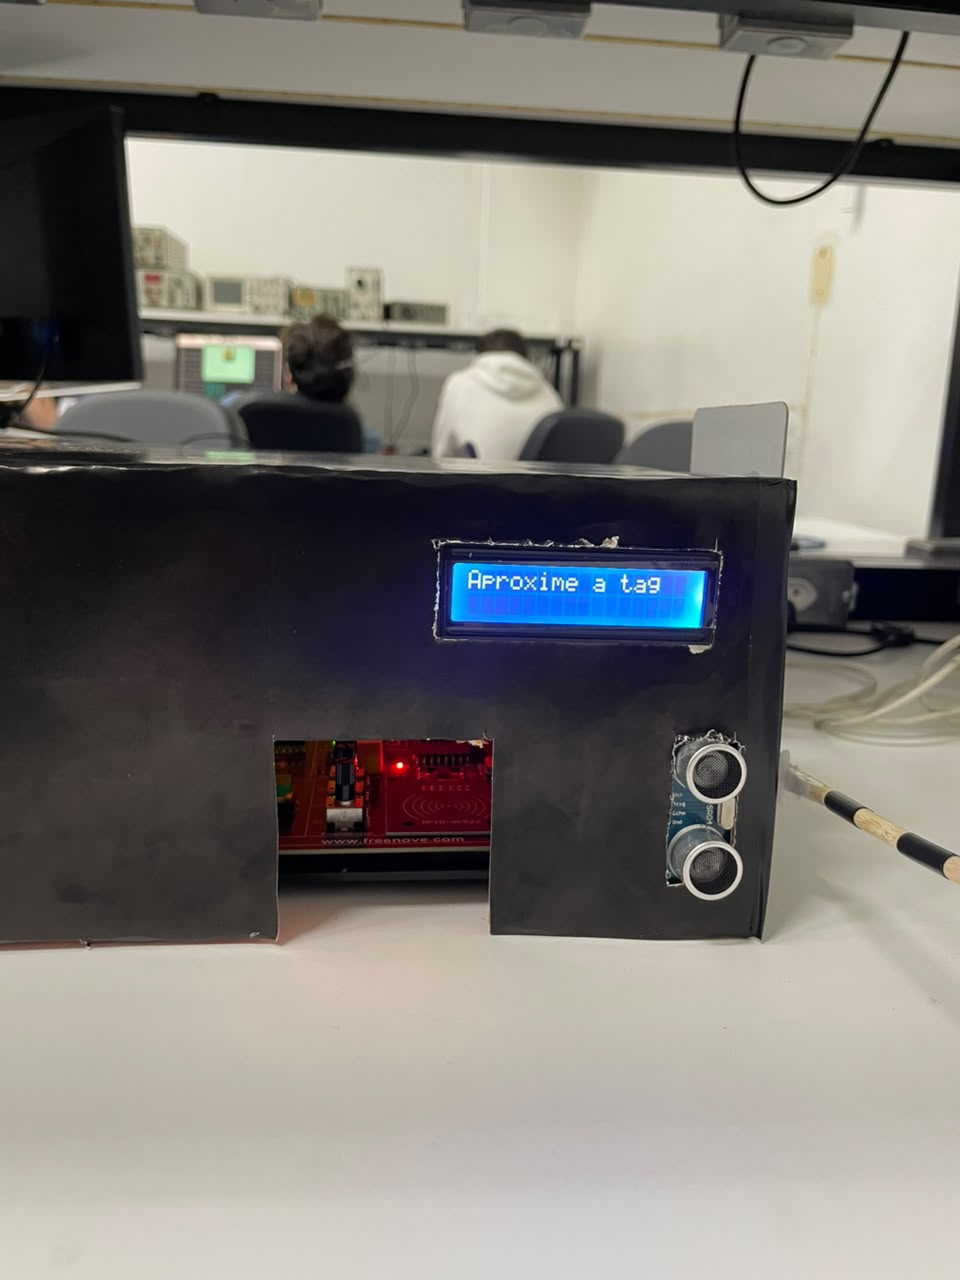
\includegraphics[width=\linewidth,height=8cm,keepaspectratio]{figuras/montagem_frontal.jpeg}
  \captionof{figure}{Vista frontal do protótipo, com o display LCD e o sensor
  ultrassônico instalados na estrutura.}
  \label{fig:montagem-frontal}
\end{minipage}\hfill
\begin{minipage}{0.48\textwidth}
  \centering
  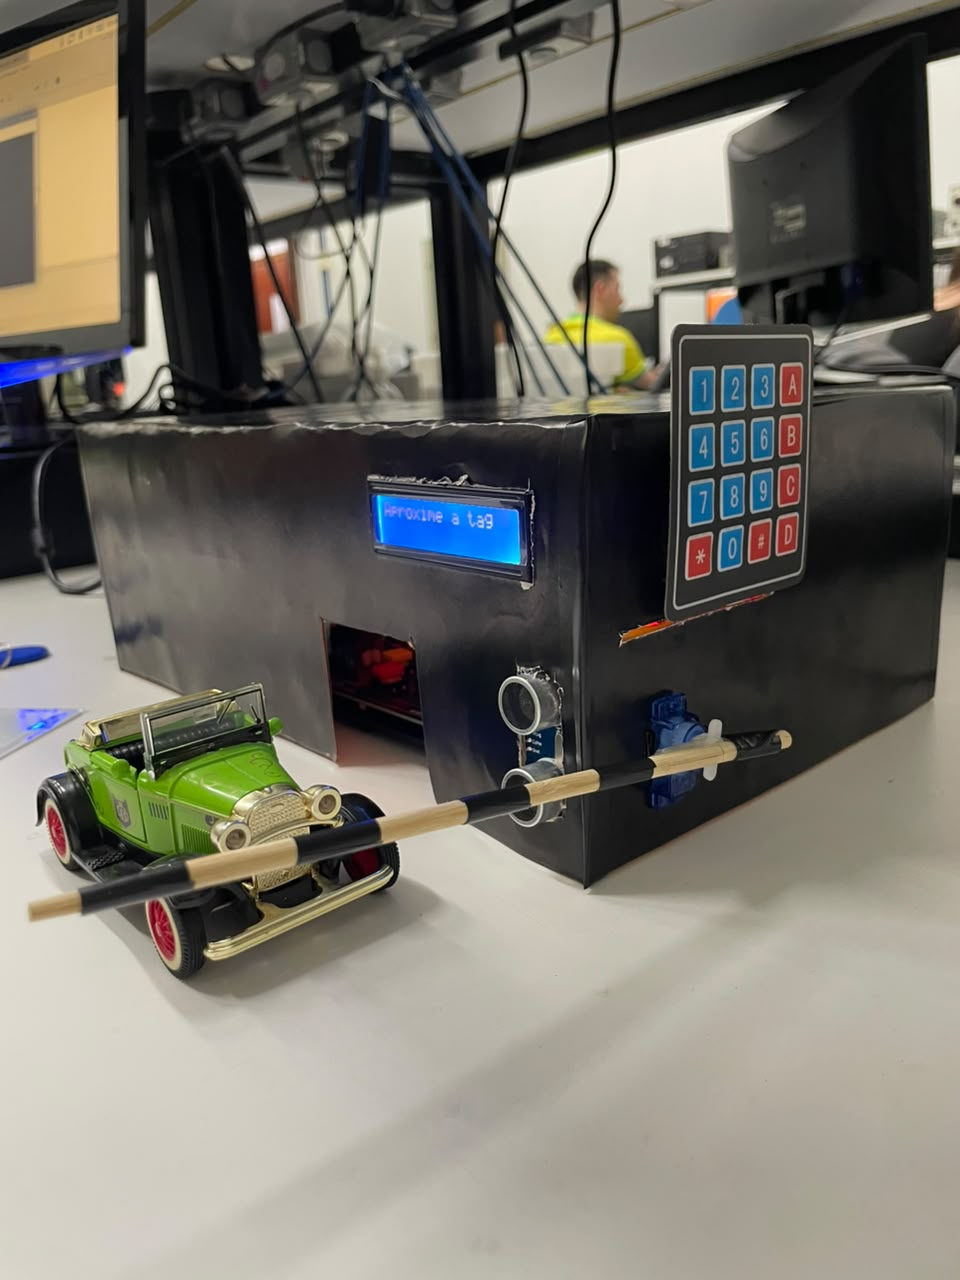
\includegraphics[width=\linewidth,height=8cm,keepaspectratio]{figuras/montagem_perspectiva.jpeg}
  \captionof{figure}{Vista em perspectiva da montagem completa, mostrando o
  teclado, a cancela acionada pelo servomotor e o veículo utilizado nos testes.}
  \label{fig:montagem-geral}
\end{minipage}
\end{figure}



% =====================================================================
\section{Resultados}
% =====================================================================

Os testes funcionais foram conduzidos em bancada com as tags cadastradas, o
teclado matricial, o sensor ultrassônico, o LCD e a cancela simulada pelo
servomotor. Para validar o comportamento noturno, o horário considerado pelo
programa foi ajustado para a faixa em que o segundo fator é obrigatório. A
passagem do veículo foi simulada com o carrinho utilizado na montagem física,
mantendo-o ou retirando-o da região monitorada pelo HC-SR04 conforme o cenário
avaliado.

Como não foi adotado um protocolo estatístico com número fixo de repetições para
cada cenário, os resultados são apresentados de forma funcional, indicando se o
comportamento esperado foi observado durante a integração e demonstração do
protótipo.

\begin{table}[H]
\centering
\small
\caption{Resultados dos casos de teste funcionais.}
\label{tab:testes}
\begin{tabular}{@{}lL{5.7cm}L{5.5cm}L{2.0cm}@{}}
\toprule
\textbf{ID} & \textbf{Cenário} & \textbf{Resultado esperado} &
\textbf{Situação} \\
\midrule
CT01 & Tag válida, período diurno
& Cancela abre sem solicitar senha
& Validado \\[3pt]

CT02 & Tag não cadastrada
& Acesso negado e cancela permanece fechada
& Validado \\[3pt]

CT03 & Tag válida e senha correta, período noturno
& Cancela abre após o segundo fator
& Validado \\[3pt]

CT04 & Três tentativas de senha incorreta
& Acesso bloqueado e cancela permanece fechada
& Validado \\[3pt]

CT05 & Senha não confirmada dentro do tempo limite
& \textit{Timeout} e acesso negado
& Validado \\[3pt]

CT06 & Obstáculo mantido na região do sensor
& Cancela não fecha enquanto a área estiver ocupada
& Validado \\[3pt]

CT07 & Ausência de resposta válida do sensor
& Fechamento não é executado sem confirmação de área livre
& Validado \\[3pt]

CT08 & Passagem completa do veículo
& Cancela fecha somente após confirmação de área livre
& Validado \\[3pt]

CT09 & Entrada autorizada
& Veículo passa a constar no registro persistente de presença
& Validado \\[3pt]

CT10 & Nova leitura de uma tag já registrada como presente
& Operação é interpretada como saída e o LCD apresenta mensagem de despedida
& Validado \\[3pt]

CT11 & Saída concluída
& Veículo é removido do registro de presença
& Validado \\[3pt]

CT12 & Entrada ou saída autorizada
& Evento é acrescentado ao histórico com data e horário
& Validado \\[3pt]

CT13 & Reinicialização do programa com veículos registrados
& Estado de presença é recuperado a partir do arquivo persistente
& Validado \\
\bottomrule
\end{tabular}
\end{table}

Os testes evidenciaram que o uso conjunto do RFID e do arquivo de presença é
suficiente para distinguir os dois sentidos de circulação no protótipo com uma
única cancela. A persistência também eliminou um problema presente em versões
iniciais: o estado dos veículos não depende mais exclusivamente de variáveis em
memória e pode ser recuperado após uma nova execução do programa.

No mecanismo de segurança física, o comportamento adotado é conservador. A
cancela somente inicia o fechamento após leituras sucessivas indicando que a
área está livre. Leituras inválidas ou ausência de eco não são interpretadas
como confirmação de passagem, evitando que uma falha do sensor seja usada como
condição para fechar a cancela sobre um veículo.

% =====================================================================
\section{Conclusão}
% =====================================================================

O sistema de controle de acesso veicular proposto foi implementado sobre uma
Raspberry Pi 3 Model B+, integrando leitor RFID, display LCD, servomotor, sensor
ultrassônico e teclado matricial. A solução realiza autenticação por RFID no
período diurno e acrescenta uma senha como segundo fator no período noturno,
mantendo a cancela fechada quando a autenticação não é concluída com sucesso.

Além do fluxo de autenticação e acionamento, a versão final incorpora
armazenamento persistente. O sistema mantém um registro dos veículos atualmente
presentes no estacionamento e utiliza essa informação para interpretar uma nova
leitura da mesma tag como saída. Após a entrada, o veículo é acrescentado ao
registro; após a saída, é removido. Um segundo arquivo mantém o histórico
cumulativo das entradas e saídas com data e horário, permitindo auditoria básica
dos acessos e preservando as informações entre execuções do programa.

A estratégia de desenvolvimento incremental, com validação isolada de cada
periférico antes da integração, reduziu a complexidade da depuração. Também foi
adotada uma política conservadora para o movimento da cancela: o fechamento só
é realizado quando o sensor confirma repetidamente que a área de passagem está
livre. Dessa forma, uma leitura inválida do sensor não é tratada como indicação
de segurança para fechar a cancela.

No protótipo atual, entrada e saída são representadas pela mesma cancela física.
A identificação do sentido ocorre por software, a partir do registro de
presença. Como continuidade do trabalho, uma segunda cancela e um segundo ponto
de leitura poderiam separar fisicamente os dois fluxos. Outras evoluções
naturais são o cadastro dinâmico de tags, o armazenamento protegido das senhas,
a substituição dos arquivos texto por um banco de dados em aplicações de maior
escala e a inclusão do buzzer previsto como sinalização opcional.

A principal limitação da persistência em arquivos texto é a ausência de
mecanismos próprios para acesso concorrente e transações. Essa escolha é
adequada ao protótipo de uma única Raspberry Pi e uma única cancela, mas não
seria suficiente, sem adaptações, para uma instalação com vários pontos de
entrada e saída operando simultaneamente. Ainda assim, para os objetivos
didáticos do projeto, a solução final demonstra de forma integrada a interação
entre interfaces SPI, I\textsuperscript{2}C e GPIO, controle por software,
sensoriamento físico, autenticação e persistência de dados.

% =====================================================================
%  BIBLIOGRAFIA (arquivo externo: referencias.bib)
% =====================================================================

\bibliographystyle{plainnat}
\renewcommand{\bibname}{Referências}
\renewcommand{\refname}{Referências}
\bibliography{referencias}
\addcontentsline{toc}{section}{Referências}

\end{document}
